\chapter{Implementation code}

The implementation can also be found on Github: \href{https://github.com/robinno/refGenMapping}{https://github.com/robinno/refGenMapping}

\section{Filesystem organization}

To keep the code manageable, it was split up in multiple files. These files were organized in the directory structure as seen in figure \ref{fig:dirStruct}

\begin{figure}[H]
	\centering
	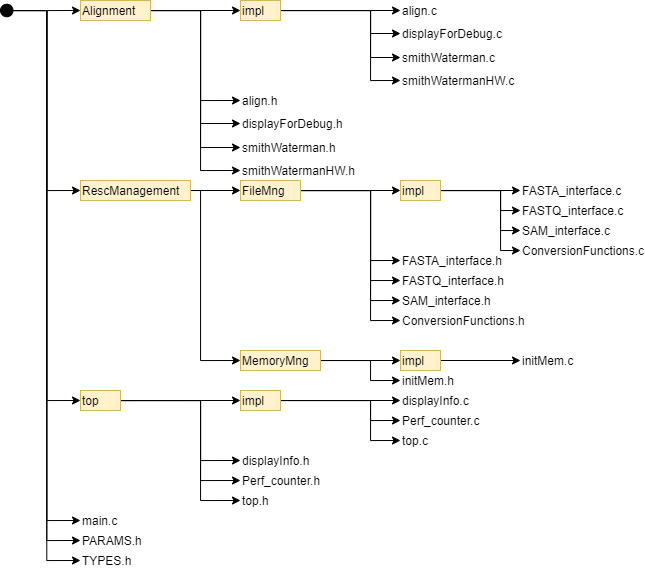
\includegraphics[width=0.8\textwidth]{code/dirStructure.png}
	\caption{The used directory structure in the implementation. Directories are colored in yellow.}
	\label{fig:dirStruct}
\end{figure}

\section{Code}
%listing all code files

{\setstretch{1.0} %interlinie afstand
	
\textbf{PARAMS.h}
\lstinputlisting[language=C]{sourceCode/PARAMS.h}
\textbf{TYPES.h}
\lstinputlisting[language=C]{sourceCode/TYPES.h}
\textbf{main.c}
\lstinputlisting[language=C]{sourceCode/main.c}


\textbf{top.h}
\lstinputlisting[language=C]{sourceCode/top/top.h}
\textbf{top.c}
\lstinputlisting[language=C]{sourceCode/top/impl/top.c}
\textbf{displayInfo.h}
\lstinputlisting[language=C]{sourceCode/top/displayInfo.h}
\textbf{displayInfo.c}
\lstinputlisting[language=C]{sourceCode/top/impl/displayInfo.c}
\textbf{Perf\_counter.h}
\lstinputlisting[language=C]{sourceCode/top/Perf_counter.h}
\textbf{Perf\_counter.c}
\lstinputlisting[language=C]{sourceCode/top/impl/Perf_counter.c}


\textbf{ConversionFunctions.h}
\lstinputlisting[language=C]{sourceCode/RescManagement/FileMng/ConversionFunctions.h}
\textbf{ConversionFunctions.c}
\lstinputlisting[language=C]{sourceCode/RescManagement/FileMng/impl/ConversionFunctions.c}
\textbf{FASTA\_interface.h}
\lstinputlisting[language=C]{sourceCode/RescManagement/FileMng/FASTA_interface.h}
\textbf{FASTA\_interface.c}
\lstinputlisting[language=C]{sourceCode/RescManagement/FileMng/impl/FASTA_interface.c}
\textbf{FASTQ\_interface.h}
\lstinputlisting[language=C]{sourceCode/RescManagement/FileMng/FASTQ_interface.h}
\textbf{FASTQ\_interface.c}
\lstinputlisting[language=C]{sourceCode/RescManagement/FileMng/impl/FASTQ_interface.c}
\textbf{SAM\_interface.h}
\lstinputlisting[language=C]{sourceCode/RescManagement/FileMng/SAM_interface.h}
\textbf{SAM\_interface.c}
\lstinputlisting[language=C]{sourceCode/RescManagement/FileMng/impl/SAM_interface.c}


\textbf{initMem.h}
\lstinputlisting[language=C]{sourceCode/RescManagement/MemoryMng/initMem.h}
\textbf{initMem.c}
\lstinputlisting[language=C]{sourceCode/RescManagement/MemoryMng/impl/initMem.c}


\textbf{align.h}
\lstinputlisting[language=C]{sourceCode/Alignment/align.h}
\textbf{align.c}
\lstinputlisting[language=C]{sourceCode/Alignment/impl/align.c}
\textbf{displayForDebug.h}
\lstinputlisting[language=C]{sourceCode/Alignment/displayForDebug.h}
\textbf{displayForDebug.c}
\lstinputlisting[language=C]{sourceCode/Alignment/impl/displayForDebug.c}
\textbf{smithWaterman.h}
\lstinputlisting[language=C]{sourceCode/Alignment/smithWaterman.h}
\textbf{smithWaterman.c}
\lstinputlisting[language=C]{sourceCode/Alignment/impl/smithWaterman.c}
\textbf{smithWatermanHW.h}
\lstinputlisting[language=C]{sourceCode/Alignment/smithWatermanHW.h}
\textbf{smithWatermanHW.c}
\lstinputlisting[language=C]{sourceCode/Alignment/impl/smithWatermanHW.c}
} %end line stretch


